\documentclass[thesis.tex]{subfiles}

\begin{document}
\iffulldocument\else
	\chapter{KdV5}
\fi

\section{Introduction}

\subsection{Background}

The Kawahara equation, also known as a fifth-order KdV-type equation, is used as a model for capilary-gravity water waves, magneto-acoustic waves, plasma waves, and other dispersive phenomena. This equation takes the general form
\begin{equation}\label{kawahara}
u_t + \alpha u_{xxx} + \beta u_{xxxxx} = \frac{\partial}{\partial x} f(u, u_x, u_{xxx}),
\end{equation}
where $u(x, t)$ is a real-valued function, the parameters $\alpha$ and $\beta$ are real with $\beta \neq 0$, and $f$ is a smooth function \cite{Bridges2002,Bridges2002a}. If $f$ is a variational derivative, then \eqref{kawahara} is the Hamiltonian system
\[
\partial_t u = \calJ \calE'(u)
\]
where $\calJ = \partial_x$ is skew-Hermitian, and the energy $\calE$ is given by
\[
\calE(u) = -\frac{1}{2}\int_{-\infty}^\infty 
\left( \frac{1}{2}u_{xx}^2 - \frac{1}{2}\alpha + u_x^2 + h(u, u_x, u_{xx})\right)dx,
\]
where $f$ is the variational derivative of the term involving $h$ \cite{Bridges2002}.

One specific example is the following PDE
\begin{equation}\label{capgrav}
u_t + \frac{2}{15} \beta u_{xxxxx} - b u_{xxx}
+ 3 u u_x + 2 u_x u_{xx} + u u_{xxx} = 0,
\end{equation}
which is a weakly nonlinear long-wave approximnation to the classical capillary-gravity water wave problem \cite{Sandstede2013,Champneys1997,Champneys1998}. Equation \eqref{capgrav} is the Kawahara equation with $\alpha = -b$, $\beta = 2/15$, and $f(u, u_x, u_{xx}) = -(\frac{3}{2}u^2 + u u_{xx} + u_x^2)$.

For simplicity, we will consider form of the Kawahara equation from \cite{Pelinovsky2007}, which we will refer to as the 5th order KdV equation (KdV5).
\begin{equation}\label{KdV5}
u_t = u_{xxxxx} - u_{xxx} - 2 u u_x 
\end{equation}
This is the Kawahara equation with $\alpha = 1$, $\beta = -1$, and $f(u, u_x, u_{xx}) = u^2$. We are interested in traveling wave solutions, which are solutions of the the form $u = \phi(x - ct)$. Writing this in a co-moving frame with speed $c$ by letting $\xi = x - ct$, equation \cref{KdV5} becomes
\begin{equation}\label{KdV5c}
u_t = \partial_x(u_{xxxx} - u_{xx} - u^2 + cu) 
\end{equation}
where we have renamed the independent variable back to $x$. Equation \cref{KdV5c} is Hamiltonian, and can be written as $u_t = \partial_x \calE'(u)$, where $\calE(u)$ is the energy
\begin{equation}\label{KdV5energy}
\calE(u) = -\int_{-\infty}^{\infty} \left( \frac{1}{2}u_{xx}^2 + \frac{1}{2}u_x^2 + \frac{1}{2}cu^2 - \frac{1}{3}u^3 \right) dx
\end{equation}
For any solution $u(x, t)$ to \cref{KdV5c}, the energy $\calE(u)$ is conserved in $t$. Since $\calE(u)$ only depends on the independent variable $x$ via $u(x)$, the energy is translation invariant. Finally, $\calE(u)$ is reversible, i.e. is invariant under the transformation $x \mapsto -x$.

An equilibrium solution to \cref{KdV5} satisfies the 5th order nonlinear ODE
\begin{equation}\label{KdV5eq}
u_{xxxxx} - u_{xxx} + c u_x - 2 u u_x = 0
\end{equation}
The background state $u = 0$ is a solution to \cref{KdV5eq}. We are interested in pulse solutions, which are localized solutions which decay exponentially to the background state at $\pm \infty$. Integrating \cref{KdV5eq} once, a pulse solution must also satisfy the 4th order ODE
\begin{equation}\label{KdV5eq4}
u_{xxxx} - u_{xx} + c u - u^2 = 0,
\end{equation}
where we take the constant of integration to be 0 since pulse solutions decay to 0. Equation \cref{KdV5eq4} is Hamiltonian, with energy given by
\begin{equation}\label{KdV5ham}
H(u, u_x, u_{xx}, u_{xxx}) = u_x u_{xxx} - \frac{1}{2}u_x^2 - \frac{1}{2}u_{xx}^2 + \frac{c}{2}u^2 - \frac{1}{3}u^3 
\end{equation}
For any solution $u(x)$ to \cref{KdV5eq4}, the Hamiltonian $H$ is conserved in $x$. 

We can write \cref{KdV5eq4} in standard Hamiltonian form as the first order system in $\R^4$
\begin{equation}\label{KdV5ham2}
Q' = (J \nabla \tilde{H}) Q,
\end{equation}
where 
\begin{equation}\label{KdV5Q}
Q = (q_1, q_2, p_1, p_2) = (u, u_x, -u_{xxx} + u_x, u_{xx}),
\end{equation}
\begin{equation}
\tilde{H}(q_1, q_2, p_1, p_2) = \frac{1}{3}q_1^3 - \frac{1}{2}c q_1^2 + p_1 q_2 - \frac{1}{2}q_2^2 + \frac{1}{2}p_2^2,
\end{equation}
and $J$ is the standard $4 \times 4$ symplectic matrix
\[
J = \begin{pmatrix}
0 & I_2 \\ -I_2 & 0
\end{pmatrix},
\]
where $I_2$ is the $2\times 2$ identity matrix. This form is particularly useful for numerical analysis.

Linearization of the 4th order ODE \cref{KdV5eq4} about a solution $u^*(x)$ is the self-adjoint linear operator
\begin{equation}\label{KdV5hessian}
\calE''(u^*) = \partial_x^4 - \partial_x^2 + c - 2 u^* 
\end{equation}
where $\calE''(u^*)$ is the Hessian of the energy \cref{KdV5energy}. For the rest state $u^* = 0$, the eigenvalues of $\calE''(u^*)$ are the solutions to the fourth-order polynomial equation $\nu^4 - \nu^2 + c = 0$, which are
\begin{align*}
\nu = \pm \sqrt{ \frac{1 \pm \sqrt{1 - 4c} }{2}}.
\end{align*}
For $c > 0$, two eigenvalues have positive real part and two have negative real part, thus $u = 0$ is a hyperbolic equilibrium with a two-dimensional stable manifold and a two-dimensional unstable manifold. For $0 < c < 1/4$, all four eigenvalues are real. A bifurcation takes place at $c = 1/4$, and for $c > 1/4$, the eigenvalues of $\calE''(0)$ are a quartet $\pm \alpha_0 \pm \beta_0 i$, where $\alpha_0, \beta_0 > 0$. This is shown in \cref{fig:kdv5eigbif}.

\begin{figure}[H]
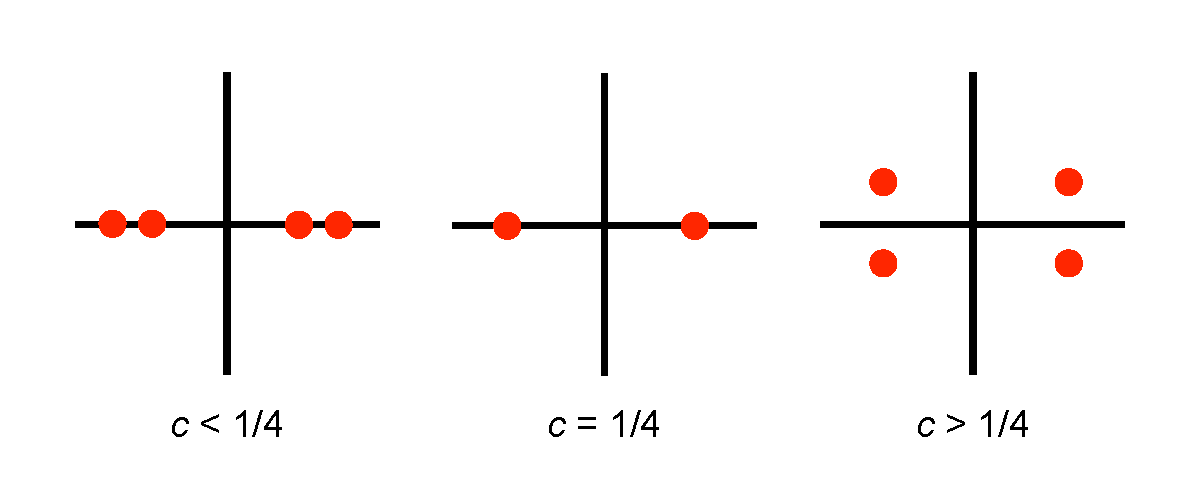
\includegraphics[width=10cm]{images/kdv5/A0eigbifurcation}
\caption{Eigenvalue pattern for linearization of \cref{KdV5eq4} about the rest state $u = 0$. }
\label{fig:kdv5eigbif}
\end{figure} 

For an equilibrium solution $u^*$, substituting the standard linearization ansatz $u(x, t) = u^*(x) + \epsilon e^{\lambda t} v(x)$ into the PDE \eqref{KdV5c} and keeping terms up to order $\epsilon$ yields the PDE eigenvalue problem
\begin{equation}\label{KdV5PDEevp}
\partial_x \calE''(u^*) v = \lambda v.
\end{equation}
where
\begin{equation}\label{KdV5PDEevpop}
\calE''(u^*) = \partial_x(\partial_x^4 - \partial_x^2 + c - 2 u^*)
\end{equation}

\subsection{Single and multi-pulses}

For $c > 0$, a symmetric one-pulse solution exists to \cref{KdV5eq4}. We will refer to this as the primary pulse solution. This result is stated in the following theorem, which is adapted from \cite[Theorem 2.1]{Pelinovsky2007}.

\begin{theorem}[Existence of Primary Pulse]\label{KdV1pulse}
For $c > 0$, there exists a one-pulse solution $q(x; c)$ to \cref{KdV5eq4} which is an even function and decays exponentially to 0 at $\pm \infty$. For the linear operators $\calE''(q)$ and $\partial_x \calE''(q)$, we have the following:
\begin{enumerate}[(i)]
\item The linear operator $\calE''(q)$ has exactly one negative eigenvalue with an even eigenfunction and a simple eigenvalue at 0 with eigenfunction $q_x$.
\item Assume that the map $c \mapsto q(x; c)$ is $C^1$ for $c > 0$. Then the linear operator $\partial_x \calE''(q)$ has an eigenvalue at 0 with algebraic multiplicty 2 and geometric multiplicty 1; the eigenfunction is $q_x$ and the generalized eigenfunction is $q_c$. 
\item Assume that 
\[
\frac{\partial}{\partial c} \left( \frac{1}{2} \int_{-\infty}^\infty q(x; c)^2 dx \right) > 0
\]
Then $q(x; c)$ is orbitally stable. This implies that $\partial_x \calE''(q)$ has no eigenvalues with positive real part.
\end{enumerate}
\end{theorem}

For $c > 1/4$, multi-pulse solutions exist to \cref{KdV5eq4}. These resemble multiple, well-separated copies of the primary pulse $q(x)$. Heuristically, we construct a multi-pulse by glueing together multiple copies of the primary pulse end-to-end. This is shown in \cref{fig:multipulsediag}.

\begin{figure}[H]
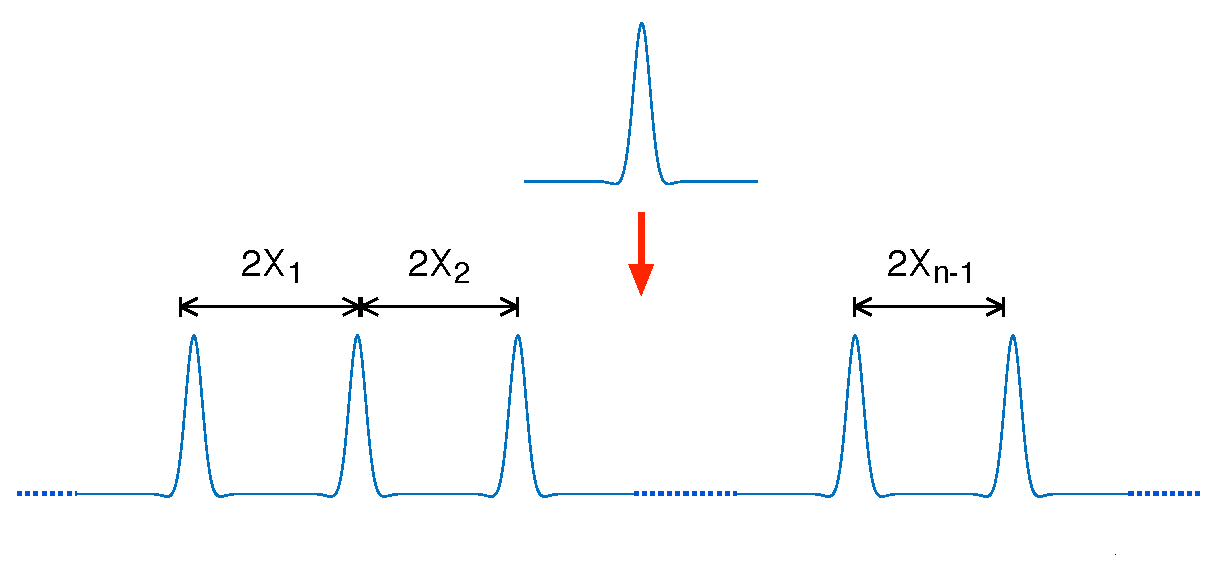
\includegraphics[width=12cm]{images/kdv5numerics/multipulse.eps}
\caption{Construction of a multi-pulse solution from the primary pulse.}
\label{fig:multipulsediag}
\end{figure}

An $n$-pulse can be characterized by $n-1$ lengths $\{ X_1, \dots, X_{n-1} \}$, where the distance between consecutive peaks is $2 X_j$. For each $n \geq 2$, a countable family of multi-pulse solutions exists \cite{Buffoni1996,SandstedeStrut}. Rather than using describing a multi-pulse by the pulse distances, we will use the parameterization from \cite{SandstedeStrut}, which is more mathematically convenient. An $n-$pulse be described using the following parameters:
\begin{enumerate}
\item A scaling parameter $r \in \calR$ with $r > 0$, where
\[
\calR = \left\{ \exp\left(-\frac{2 \pi \alpha_0}{\beta_0}m \right) : m \in \N_0 \right\}
\]
\item A sequence of $n-1$ baseline length parameters $\{ b_1^0, \dots, b_{n-1}^0 \}$, where 
\[
b_j = \exp\left(-\frac{\pi \alpha_0}{\beta_0}m_j \right)
\]
for $m_j \in \N_0$, and we have the additional restriction that $m_j \in \{0, 1\}$ for some $j$.
\end{enumerate}

The following theorem, which is adapted from \cite[Theorem 3.6]{SandstedeStrut} states the existence result for multi-pulse solutions.

\begin{theorem}[Existence of Multi-Pulses]\label{KdVmultipulse}
There exists $\delta > 0$ such that for any $n \geq 2$ the following holds. For any sequence of baseline length parameters $\{ b_1^0, \dots, b_{n-1}^0 \}$, there exists $r_0 \in \calR$, $r_0 > 0$ with the following property.
\begin{enumerate}[(i)]
\item For every scaling parameter $r \in \exp\left(-\frac{2 \pi \alpha_0}{\beta_0}m \right) \in \calR$ with $0 < r \leq r_0$ there exists a unique $n$-pulse solution $q_n$ which resembles $n$ consecutive copies of $q$. The distances between consecutive peaks are given by
\[
X_j = \frac{\pi}{\beta_0}(2 m + m_j) + R_j(r) + \tilde{L}
\]
where $\tilde{L}$ is a constant and the remainder terms $R_j(r) \rightarrow 0$ as $r \rightarrow 0$.
\item There are exactly $n$ real eigenvalues $\lambda_j$ of $\calE''(q_n)$ with $|\lambda_j| < \delta$. These are as follows.
\begin{enumerate}
	\item There are $n_{\text{odd}}$ negative eigenvalues, where $n_{\text{odd}}$ is the number of $m_j$ which are odd.
	\item There are $n_{\text{even}}$ positive eigenvalues, where $n_{\text{even}}$ is the number of $m_j$ which are even.
	\item There is a simple eigenvalue at 0 with corresponding eigenfunction $\partial_x q_n$.
\end{enumerate}
\end{enumerate}
\begin{proof}
For $c > 1/4$, the eigenvalues of $\calE''(0)$ are a quartet $\pm \alpha_0 \pm \beta_0$. Equation \cref{KdV5eq4} is Hamiltonian, with conserved quantity \cref{KdV5ham2}. The relevant Melnikov integral is
\[
M = \int_{-\infty}^\infty q(x)^2 dx > 0
\]
Thus Hypotheses 3.1, 3.3, and 3.5 in \cite{SandstedeStrut} are satisfied. The result follows from \cite[Theorem 3.6]{SandstedeStrut}. Since $\calE''(q_n)$ is self-adjoint, its eigenvalues are real.
\end{proof}
\end{theorem}

We remark that spectral stability of a multipulse solution $q_n$ will depend on the parity of the length pararemers $b_j^0$ used to construct the multipulse. Geometrically, these represent the number of half-twists made by $q_n(x)$ near the equilbrium at 0 between consecutive peaks \cite{SandstedeStrut}. Although we will not need the eigenvalue result from part (ii) of \cref{KdVmultipulse}, it is relatively straightforward to determine the spectrum of $\calE''(q_n)$ numerically; determining the length parameters $b_j^0$ may be more difficult.

\subsection{Spectral stability}

We now turn to the spectral stabilty problem for a multipulse $q_n$. To do this, we study the spectrum of the linearization $\partial_x \calE''(q_n)$. It it straightforward to show that 
\begin{align*}
\partial_x \calE''(q_n) (\partial_x q_n) &= 0 \\
\partial_x \calE''(q_n) (-\partial_c q_n) &= \partial_x q_n
\end{align*}
For the essential spectrum, since \cref{KdV5PDEevpop} is exponentially asymptotic to the operator 
\[
\partial_x \calE''(0) = 
\partial_x(\partial_x^4 - \partial_x^2 + c - 2 u^*),
\]
by the Weyl essential spectrum theorem \cite[Theorem 2.2.6]{Kapitula2013} and \cite[Theorem 3.1.11]{Kapitula2013}, $\partial_x \calE''(q_n)$ and $\partial_x \calE''(0)$ have the same essential spectrum. By a straightforward calculation, the essential spectrum of $\partial_x \calE''(q_n)$ is the entire imaginary axis.

It remains to locate the rest of the point spectrum. To do this, we write the PDE eigenvalue problem \cref{KdV5PDEevp} as the first order system in $\R^5$
\begin{equation}\label{KdV5PDEevp2}
V'(x) = A(q_n(x))V(x) + \lambda B V(x),
\end{equation}
where
\begin{align*}
A(q_n(x)) &= \begin{pmatrix}0 & 1 & 0 & 0 & 0 \\0 & 0 & 1 & 0 & 0 \\0 & 0 & 0 & 1 & 0 \\0 & 0 & 0 & 0 & 1 \\
2 \partial_x q_n(x) & 2 q_n(x) - c & 0 & 1 & 0 \end{pmatrix}, &&
B = \begin{pmatrix}0 & 0 & 0 & 0 & 0 \\0 & 0 & 0 & 0 & 0 \\0 & 0 & 0 & 0 & 0 \\0 & 0 & 0 & 0 & 0 \\
1 & 0 & 0 & 0 & 0 \end{pmatrix} \\
\end{align*}
The matrix $A(q_n(x))$ is exponentially asymptotic to the constant coefficient matrix $A(0)$, which as eigenvalues $\{ 0, \pm \alpha_0 \pm \beta_0 \}$. Since $A(0)$ is not hyperbolic, we cannot directly apply the results of \cite{Sandstede1998}. 

We expect that, as in \cite{Sandstede1998}, an additional eigenvalue near 0 will be associated with each additional pulse. We will call these interaction eigenvalues. Since \cref{KdV5c} is Hamiltonian, these interaction eigenvalues must come in quartets $\{ \pm \lambda, \pm \overline{\lambda}\}$ \cite[Proposition 5.1.2]{Kapitula2013}. Thus we expect that each additional pulse will be associated with a set of eigenvalues which must come in one of the three patterns in \cref{fig:kdv5inteigpattern}.

\begin{figure}[H]
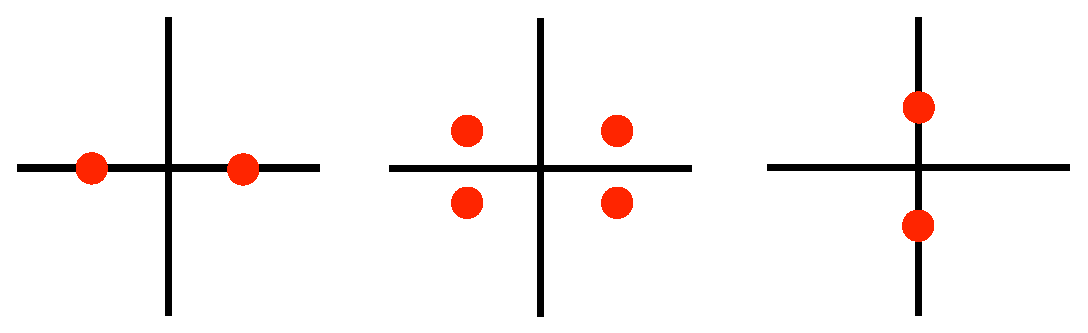
\includegraphics[width=10cm]{images/kdv5/eigdouble2}
\caption{Possible interaction eigenvalue patterns for multipulses for KdV5. The first two patterns are unstable. The third pattern is neutrally stable.}
\label{fig:kdv5inteigpattern}
\end{figure}

By Hamiltonian symmetry, the presence of an eigenvalue with nonzero real part implies that there is an unstable eigenvalue with positive real part. Thus the best we can hope for is neutral stability.

For double pulses, we have the following result due to Chugunova and Pelinovsky \cite{Pelinovsky2007}.

\begin{theorem}\label{KdV5doubleeigs}
Let $q_2(x)$ be a double pulse solution constructed with length parameter $b_1^0 = e^{-\frac{\pi \alpha_0}{\beta_0}m_1}$. Let $\nu$ be the small, nonzero eigenvalue of $\calE''(q_2)$ from \cref{KdVmultipulse}(ii).
Then
\begin{enumerate}[(i)]
	\item If $m_1$ is even (equivalently, $\nu > 0)$, the operator $\partial_x \calE''(q_2)$ has a pair of real eigenvalues.
	\item If $m_1$ is odd (equivalently, $\nu < 0)$, the operator $\partial_x \calE''(q_2)$ has a pair of eigenvalues which are purely imaginary to leading order.
\end{enumerate}
\begin{proof}
This is part (iii) of \cite[Theorem 2.3]{Pelinovsky2007}, where we note that $W''(L_n) > 0$ corresponds to $m_1$ odd and $W''(L_n) < 0$ corresponds to $m_1$ even.
\end{proof}
\end{theorem}

\iffulldocument\else
	\bibliographystyle{amsalpha}
	\bibliography{thesis.bib}
\fi

\end{document}